\chapter{Introduction}
\lettrine[lines=2, findent=3pt, nindent=0pt]{I}{}n the frame of astronomical spectroscopy...

\bigskip
In \hyperref[chap:1]{Chapter~\ref*{chap:1}} we  briefly present...

\bigskip
In \hyperref[chap:2]{Chapter~\ref*{chap:2}} we summarize...
\section{Motivations}
\section{Background}
To understand better all the methods, we should do some refresh of what we will encounter during the lecture. The main arguments we should consider are \textbf{Graphs}, \textbf{Classification} and \textbf{Connectomes}.
\paragraph{Graphs}\
\\
There are many subjects in which graphs are used, and consequently many definitions. In mathematics, a graph is a structured set of objects that, in pairs, could have a relation between themselves. Each object is called a \textit{vertex}, and each relation between a pair of vertices is called an \textit{edge}. So, a graph $ G(V,E) $ is a pair where $ V $ are the vertices and $ E $ are the edges. Graphs are represented in diagram form, where vertices are in circle form and edges are lines that join pairs of vertices with a relation.
\begin{figure}[htbp]
	\centering
	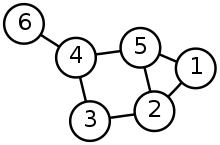
\includegraphics[scale=0.5]{Immagini/220px-6n-graf.svg.png}
	\caption{\label{fig:diagram}}
\end{figure}
\\
Graph could be \textit{directed} or \textit{undirected}. In a direct graph, edges have an orientation, the links between vertices can be represented by arrows going from one vertex to the other. In an edge $ (x,y) $ directed from $ x $ to $ y $, the vertices are called respectively \textit{tail} and \textit{head} of the edge.
\begin{figure}[htbp]
	\centering
	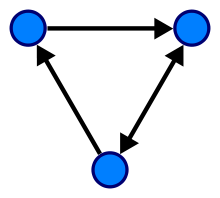
\includegraphics[scale=0.5]{Immagini/220px-Directed.svg.png}
	\caption{\label{fig:diagram2}}
\end{figure}


\section{Related works}
\section{Outline}